% flatex input: [paper.tex]
% flatex input: [./include/start.tex]
\documentclass{sigchi}

\usepackage{url,graphicx,multirow,color,calc,ulem,threeparttable,tabularx,booktabs,enumitem,subcaption,balance,amsfonts,comment}
\usepackage[group-separator={,}]{siunitx}

% llt: Define a global style for URLs, rather that the default one
\makeatletter
\def\url@leostyle{%
  \@ifundefined{selectfont}{\def\UrlFont{\sf}}{\def\UrlFont{\small\bf\ttfamily}}}
\makeatother
\urlstyle{leo}


% To make various LaTeX processors do the right thing with page size.
\def\pprw{8.5in}
\def\pprh{11in}
\special{papersize=\pprw,\pprh}
\setlength{\paperwidth}{\pprw}
\setlength{\paperheight}{\pprh}
\setlength{\pdfpagewidth}{\pprw}
\setlength{\pdfpageheight}{\pprh}

\usepackage[pdftex]{hyperref}
\hypersetup{
  bookmarksnumbered,
  pdfstartview={FitH},
  colorlinks,
  citecolor=black,
  filecolor=black,
  linkcolor=black,
  urlcolor=black,
  breaklinks=true,
  pdfinfo={
    Title={PocketParker: Pocketsourcing Parking Lot Availability},
    Author={Anandatirtha Nandugudi, Taeyeon Ki, Carl Nuessle and Geoffrey
    Challen},
  }
}

\usepackage[absolute]{textpos}

\setlength{\TPHorizModule}{1in}
\setlength{\TPVertModule}{1in}
\textblockorigin{0.75in}{0.5in}

\usepackage[all]{hypcap}

% flatex input: [.xxxnote]
\newcommand{\XXXnote}[1]{}

% flatex input end: [.xxxnote]

% To make various LaTeX processors do the right thing with page size.
% flatex input: [.draft]


% flatex input end: [.draft]

% To make various LaTeX processors do the right thing with page size.
% flatex input: [.blue]


% flatex input end: [.blue]

% To make various LaTeX processors do the right thing with page size.
% flatex input: [common.tex]
% 16 Nov 2010 : GWA : Any special macros or other stuff for this particular
%               paper go here.
\hyphenation{Pocket-Parker}
\hyphenation{pocket-sourcing}
\newcommand{\PhoneLab}{\textsc{PhoneLab}}

% flatex input end: [common.tex]

% To make various LaTeX processors do the right thing with page size.

% flatex input end: [./include/start.tex]


\begin{document}
\date{}

\numberofauthors{1}

\author{
  \alignauthor Anandatirtha Nandugudi, Taeyeon Ki, Carl Nuessle, and Geoffrey Challen\\
  \affaddr{University at Buffalo}\\
  \email{\{ans25,tki,carlnues,challen\}@buffalo.edu}
}

\title{PocketParker: Pocketsourcing Parking Lot Availability}

\toappear{\fontfamily{ptm}\selectfont Permission to make digital or hard
  copies of all or part of this work for personal or classroom use is granted
  without fee provided that copies are not made or distributed for profit or
  commercial advantage and that copies bear this notice and the full citation
  on the first page. Copyrights for components of this work owned by others
  than the author(s) must be honored. Abstracting with credit is permitted.
  To copy otherwise, or republish, to post on servers or to redistribute to
  lists, requires prior specific permission and/or a fee. Request permissions
  from \href{mailto:permissions@acm.org}{Permissions@acm.org}.\\
  
  \href{http://ubicomp.org/ubicomp2014/}{\textit{UbiComp'14}}, September 13--17 2014, Seattle, WA, USA\\
  Copyright is held by the owner/author(s). Publication rights licensed to
  ACM.\\
  ACM 978-1-4503-2968-2/14/09$\ldots$15.00.\\
\href{http://dx.doi.org/10.1145/2632048.2632098}{http://dx.doi.org/10.1145/2632048.2632098}}

\maketitle

\ifdefined\isblue
\begin{textblock}{1}(6.4,0)
\noindent\href{http://blue.cse.buffalo.edu}{
\includegraphics[width=0.6in]{./figures/logos/blue.jpg}}
\end{textblock}
\fi

% flatex input: [abstract.tex]
\begin{abstract}
% <wc:start description="Abstract" max=150>
Searching for parking spots generates frustration and pollution. To address
these parking problems, we present \textit{PocketParker}, a crowdsourcing
system using smartphones to predict parking lot availability. PocketParker is
an example of a subset of crowdsourcing we call \textit{pocketsourcing}.
Pocketsourcing applications require no explicit user input or additional
infrastructure, running effectively without the phone leaving the user's
pocket. PocketParker detects arrivals and departures by leveraging existing
activity recognition algorithms. Detected events are used to maintain per-lot
availability models and respond to queries. By estimating the number of
drivers not using PocketParker, a small fraction of drivers can generate
accurate predictions. Our evaluation shows that PocketParker quickly and
correctly detects parking events and is robust to the presence of hidden
drivers. Camera monitoring of several parking lots as 105~PocketParker users
generated \num{10827}~events over 45~days shows that PocketParker was able to
correctly predict lot availability 94\% of the time.
% <wc:end>

\end{abstract}

\keywords{
  Smartphone sensing; Crowdsourcing; Parking
}

\category{C.2.4}{Computer-Communication Networks}{Distributed Systems}

% flatex input end: [abstract.tex]

% flatex input: [introduction.tex]
\section{Introduction}

Parking lots present a difficult search problem. Lacking enough visibility to
determine where spots are available, drivers may search fruitlessly through
lot after lot, wasting time and energy while generating harmful vehicle
emissions. And while some high-demand lots in urban areas and at airports
have been instrumented to monitor availability, the high cost of the
equipment required has prevented this approach from being widely-deployed at
many lots where drivers find themselves searching for spots, including at
university campuses and suburban shopping malls. Our own campus featuring 40
lots with over 80 entrances would cost at least \$\num{28000} to monitor even
with the least expensive research prototype~\cite{propst2012embedded} and an
order-of-magnitude more with available commercial
solutions~\cite{car-detect}. Instead of relying on additional infrastructure,
we believe a free solution is already in our pockets.

\textit{PocketParker} is a system that predicts parking lot availability
using smartphones. Unlike previous approaches, our approach requires no
additional infrastructure, no vehicle modifications, and no user interaction,
only the installation of a smartphone app. PocketParker runs unattended in
the background and uses activity transitions to detect parking lot arrivals
and departures. These are forwarded to a central server that incorporates
them into per-lot availability models. This allows PocketParker to order lots
accurately by the probability that they contain an available spot. We
consider PocketParker an example of a subset of crowdsourcing that does not
require any user input which we call \textit{pocketsourcing}.

Predicting parking availability requires accurately detecting parking events
as well as determining the effect of \textit{hidden drivers}---drivers not
using PocketParker---on lot availability. We address the first challenge with
a simple, effective, and energy-efficient event detector which uses
accelerometer data to detect vehicle arrivals and departures. The second goal
we achieve with an availability estimator that maintains a probability model
for each lot by incorporating events generated by PocketParker clients.
Parking events are used both to model arrival and departure rates and to
estimate the number of hidden drivers. One key insight is that even without
monitoring all drivers there are moments when PocketParker is certain that a
parking spot is available in a particular lot and can use this information to
assist users.

Our paper makes the following contributions. After motivating our approach
through an examination of related work, we present the design of PocketParker
in detail, describing in separate sections how PocketParker detects parking
events and maintains per-lot availability models. We then perform a thorough
evaluation of each component of PocketParker and the performance of the
system as a whole. We test our parking event detector in a controlled
environment with eight volunteers participating in ten parking scenarios. We
test our parking availability estimator with a simulator providing the
ability to experiment with a variety of parking lot configurations and
arrival and departure rates.

Finally, we test the end-to-end effectiveness of PocketParker through a field
trial involving 105~smartphones users that generated \num{10827} parking
events over 45~days. To obtain ground truth, we deployed four cameras to
monitor two parking lots over two weeks and hand-coded four days' worth of
images to measure their true availability. Our results demonstrate that
PocketParker can accurately and efficiently detect parking events and use
them to make accurate availability predictions. During the field trial it was
able to correctly predict lot availability 94\% of the time.

% flatex input end: [introduction.tex]

% flatex input: [related.tex]
\section{Motivation and Related Work} While infrastructure solutions for
monitoring lot availability exist, they are extremely expensive. The SFPark
system spent \$18 million to instrument \num{7000} street spots, or roughly
\$\num{2500} per spot~\cite{sfpark}. Surface lots are cheaper to monitor
since equipment can be deployed only at ingress-egress points, but the
technology required to do so remains expensive. The vehicle detector and
transponder required at each entrance costs \$\num{9700}~\cite{car-detect}
and programmable sign to communicate lot availability to drivers running
\$\num{49000}~\cite{mstp-park}, not including the continuing cost of
telemetry. Our campus with 40~lots and over 80~lot entrances would cost
\$\num{776000} for entrance monitors alone, and over \$2~million dollars with
lot availability signs. Even using a \$\num{350}-per-entrance research
prototype based on wireless sensor network nodes would cost \$\num{28000},
again not including the cost of communication. The prohibitive cost of these
solutions has prevented their widespread deployment, with the result that
many parking lots are still not monitored.

As smartphones have become ubiquitous, multiple apps and research projects
have attempted to harness their capabilities to aid the parking process. But
while app marketplaces such as the Google Play Store teem with
parking-related apps, these apps either do not provide real-time parking lot
availability or simply display publicly-available information. Several
research projects have attempted to address these limitations but suffer from
limitations that prevent them from scaling, requiring additional
infrastructure~\cite{5062057}, on-vehicle equipment~\cite{Mathur:2010:PDS}
vehicle-to-vehicle networking~\cite{Delot:2009:CRP, Mathur:2010:PDS}, or
onerous manual user input~\cite{Chen:2012:COS}. To the best of our knowledge,
PocketParker is the first app that can monitor parking lot availability
without interacting with users.

Most close to our work is Parksense~\cite{Nawaz:2013:PSB}, a system that
leverages the ubiquity of Wifi beacons to monitor on-street parking
availability. Our study, borne out of suburban campus locale, must cope with
alternative sensing mechanisms in the wake of no proximate Wifi signals. We
have also tuned our tracking and reporting methodology to address the
different challenges produced by lot, rather than street, parking.
ParkNet~\cite{Mathur:2010:PDS} is another system that estimates street
parking availability by using vehicles equipped an ultrasonic range finder to
detect empty street parking spots. Unlike ParkNet, PocketParker does not
require new vehicle capabilities.

PocketParker's parking detector builds on existing approaches to accurate
and energy-efficient activity recognition~\cite{Constandache:2010:DYS,
Keally:2011:PTP, Reddy:2010:UMP, Yang:2011:DDP, Wang:2009:FEE}. While our
current detector is both simple and parking-focused, continued progress in
reducing the energy overhead and increasing the accuracy of smartphone
activity recognition algorithms will improve PocketParker's performance.

% flatex input end: [related.tex]

% flatex input: [detector.tex]
\section{Event Detector}

The inputs to PocketParker's availability estimation algorithm are arrival
and departure events generated by an activity detector running unattended on
users' smartphones.  While considerable previous research has explored
activity detection using mobile sensing~\cite{Constandache:2010:DYS,
Keally:2011:PTP, Reddy:2010:UMP, Yang:2011:DDP, Wang:2009:FEE}, we designed a
custom parking event detector tailored to the goals of PocketParker. 

\begin{figure}[t]
  \centering
  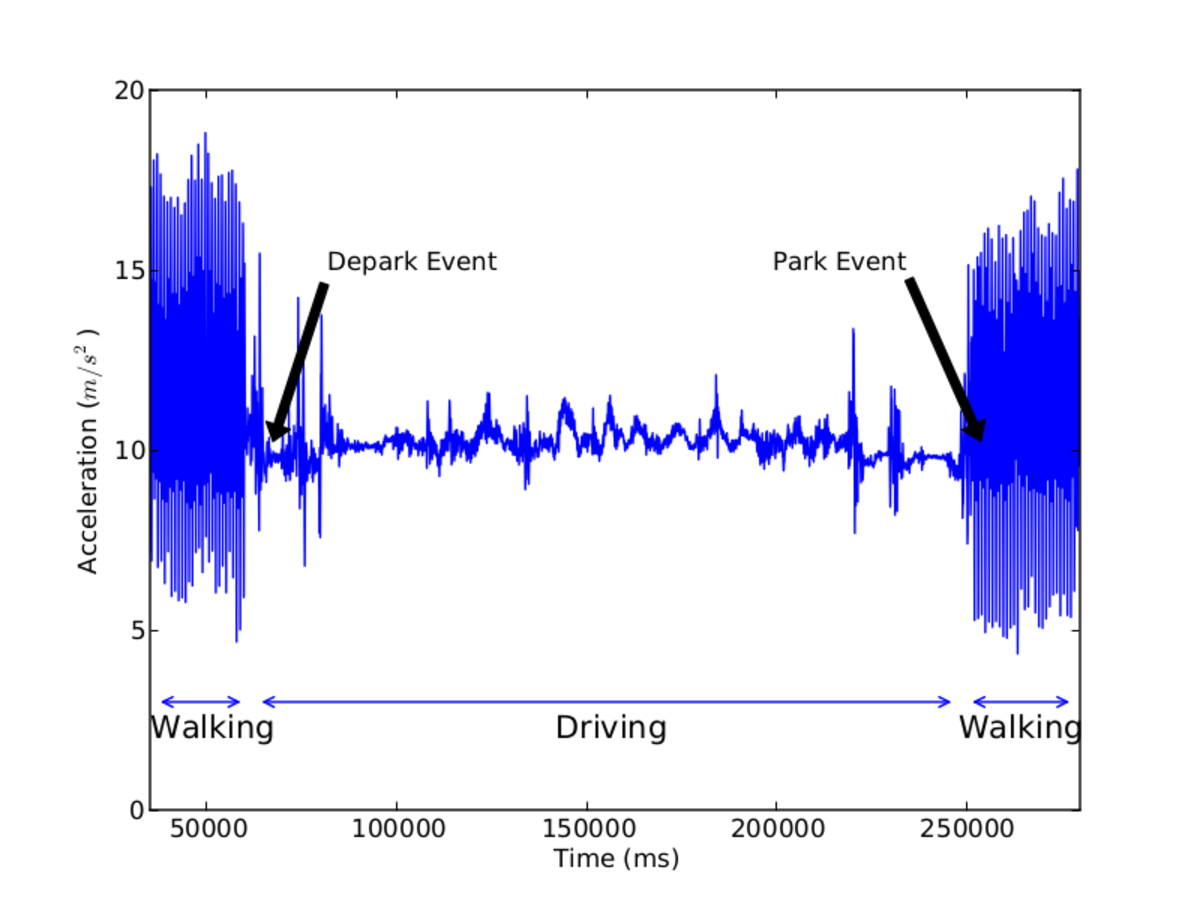
\includegraphics[width=0.8\columnwidth]{./figures/detection-cropped.pdf}

  \caption{\textbf{Detection algorithm.} The graph shows the accelerometer
    data collected during our controlled experiment and shows a period of
    walking, followed by driving, followed by a return to walking.
    Transitions between these states in areas known to be parking lots
  suggest vehicle arrivals and departures.}

  \label{fig-detection}
\end{figure}


PocketParker assumes that transitions between walking and driving that occur
inside known parking lots constitute either arrival (driving to walking) or
departure (walking to driving) events.  We thus must be able to discern
between walking and driving states of the user, and to do so fast enough to
fix the the location of the parking lot in which the event took place.
Detecting these states could be achieved using continuously-sampled GPS data
would consume too much energy for an effective pocketsourcing solution.
Rather, we rely on duty-cycled accelerometer data to classify the user
behavior into one of three states: walking, driving, or idle.

Figure~\ref{fig-detection} depicts two changes in user state, from walking to
driving and back again.  The initial inference yielded by the accelerometer
is subsequently refined with GPS and Wifi sense data to yield the desired
goal: detection of arrival and departure events.  The smartphone reports
these events and their locations to the PocketParker server. Before recording
the event, the server verifies its location against a list of known parking
lot locations to eliminate events that are either obviously incorrect (a user
parking in a field) or unwanted (a user parking but in a loading area rather
than in a lot).

After we deployed our PocketParker prototype, Google incorporated activity
recognition algorithms into its Google Play Services library. We have
incorporated them into PocketParker and, while we have not performed a
detailed evaluation, we have not found the change to affect PocketParker's
event detection accuracy.

% flatex input end: [detector.tex]

% flatex input: [model.tex]
\begin{figure}
\centering
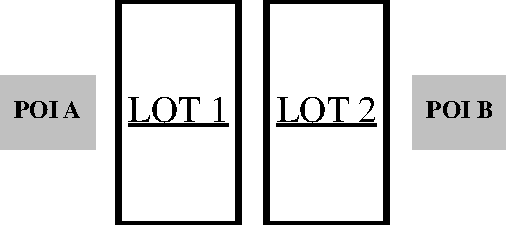
\includegraphics[width=0.6\columnwidth]{./figures/CartoonLot.pdf}

\caption{\textbf{Example parking lot setup.} Two lots and three
destinations are shown.}

\label{fig-lots}
\end{figure}

\section{Availability Estimation}

In order for parking events to be useful, they must be incorporated into a
model that allows us to predict where parking is available. Because
PocketParker focuses on monitoring surface lots, not on-street parking, we
structure our prediction engine to return the probability that a given
parking lot has space available. This information is used by drivers to
determine what lots to search and in what order. PocketParker's estimator
uses the events produced by our parking event detector both to estimate the
rates at which drivers are searching and departing from the lot and to adjust
the availability probability directly. In this section, we present both the
design of the PocketParker client parking lot availability estimator and
portions of the backend server for our system.

\subsection{Overview}

Figure~\ref{fig-lots} shows an example setup with two parking lots and two
destinations that are used throughout this section. For each lot PocketParker
maintains a time-varying probability that the lot has $n$ free spots $P(t,
n)$. While we are mainly interested in the probability that the lot has a
space available $P_{free} = \sum_{n > 0} P(t, n)$, we maintain separate
probabilities for each number of free spots so that we can manipulate
individual probabilities in response to events and queries as described
below. We bound the count probability distribution to lie between 0 and the
capacity of the parking lot. 

PocketParker's estimator receives two types of events: arrivals and
departures. However, for each arrival in a given lot, a number of additional
lots may have been searched unsuccessfully, information critical to the
accuracy of our availability model. In the next two sections we describe how
PocketParker determines relationships between parking lots and combines that
information with arrivals to estimate implicit search behavior.

Between events we want to maintain our availability model by estimating the
rate at which departures and searches are taking place. PocketParker must use
the events it can detect to estimate the rate at which events are taking
place in the lot, which includes the effect of drivers not using
PocketParker, which we call \textit{hidden drivers}. Accomplishing this
requires that we estimate the ratio between monitored and hidden drivers.
With an estimate of the hidden driver ratio, we can scale the search and
departure rates accordingly. Finally, we integrate all of this information to
update our availability estimate as arrival and departure events are
received.

\subsection{Estimating Lot Capacity}

PocketParker requires an estimate of lot capacity $C$ in several places.
First, we use this estimate to bound $P(t)$ such that $P(t, n > C) =
0\;\forall\;t$. Second, we use the capacity to determine the number of hidden
drivers. To calculate a lot capacity, we use the location of the parking lot
obtained from the OpenStreetMap database~\cite{openstreetmap}. We derive the
lot size from its location and then divide the total size by that of a
typical standard parking spot lot design~\cite{parkingdesign}. For the three
lots monitored by our deployment, capacity estimates were all within 6\% of
manually-counted ground truth. Errors in the capacity can result if the size
of parking spots in the lot differ from our estimate, or if the parking lot
is not efficiently packed with spots. Given the incentive of lot
designers to maximize capacity, we consider the second case unlikely.

\subsection{Lot Relationships}

While PocketParker's parking event detector identifies only arrivals and
departures, identifying unsuccessful searches is crucial in order to
determine the reason for a drop in arrival rates. If we observe the arrival
rate fall at a given lot, it may be because the lot is full, or it may be
simply because fewer drivers are arriving and the lot still has many spaces
available. Observing unsuccessful searches in the first case allows
PocketParker to infer that the lot is full and suggest drivers park
elsewhere. In order to estimate search behavior, we need to understand the
relationships between parking lots. This requires two additional pieces of
data about each lot: what destinations it serves and how desirable it is.

\subsubsection{Lot destinations}

The lot destination represents the place or places where the user is
ultimately going after parking. In Figure~\ref{fig-lots}, lot~1 may be
associated with destinations A, B and C; while lot~2 is only linked to B.
While mapping software can be used to assign lots to the nearest labeled
building, this approach fails when lots serve multiple destinations. To
handle this case, PocketParker uses Wifi localization of the first access
point seen by the smartphone after the user parks to determine what indoor
location the user entered after parking. The probability distribution that
emerges from a history of these events can be used to predict where a user is
going at the moment that a parking event is detected. In the future, data
from navigation tools may be able to link destinations automatically with
lots by noting where users park after requesting directions to a particular
location.

\subsubsection{Desirability index}

The desirability index reflects a lot's relative preference to drivers. We
infer a lot's desirability from the destinations associated with each lot and
the lot's distance to each, assuming that PocketParker users prefer the
closest available lot to their final destination. In Figure~\ref{fig-lots},
if lot~2 is associated with destination~A it will be ranked less desirable
than lot~1 because it is further from the destination. Integration with
navigation tools can also help refine the desirability index by observing
what lots are searched by users on their way to a particular destination.
Currently PocketParker saves energy by enabling GPS only after detecting
parking events and so does not have a trace of the users locations before
parking that could be used to identify more desirable lots.

\subsection{Implicit Searches}

With an understanding of lot relationships we can use observed arrivals to
model implicit---or unobserved---searches. When a user parks in a given lot,
we use the desirability index of the lot to add unsuccessful searches in more
desirable lots associated with the same destination. There are two challenges
to this approach. First, as described above, lots may be associated with
multiple destinations. Second, the user may not have actually performed the
search. After discussing both of these issues below, we continue by
describing how PocketParker incorporates the information from implicit
searches in a way sensitive to these uncertainties.

\subsubsection{Determining the destination}

If a lot is associated with multiple destinations, we cannot immediately
determine the user's destination.  This is not a problem as long as all
potential destinations are on the same side of the lots.  For example, in
Figure~\ref{fig-lots}, if lots 1~and~2 are both associated with destinations
A~and~C, but not with B, then an arrival with an unknown destination into lot~2
can always be used to generate an implicit search in lot~1, since the
destination does not alter the desirability ranking for the two lots.

However, having two or more destinations that are located on different sides of
lots produces an ambiguity.  If both lots~1~and~2 are associated with all
destinations, then an arrival in lot~2 cannot be resolved directly. If the
user's destination was A, it may mean that lot~1 was searched and is full.
If the destination was B, the parking event may not indicate anything about
lot~1. To resolve this ambiguity, PocketParker uses information about the users
final destination gathered as described above.

\subsubsection{Speculative searches}

If we do not directly observe a user searching a lot before we detect an
arrival, we cannot be certain that they performed the search. If the unsearched
but preferable lot was available, they may not have searched it because they
preferred to choose the first available spot, enjoyed the exercise of walking
farther to their destination. However, these are not the type of users we
believe would benefit from or use PocketParker, since finding a
non-optimal parking spot is fairly simple in most cases.

A more interesting case is where a user has not performed a search in a
desirable lot because it \textit{looks} full. Users that park regularly at
the same destination may maintain temporal models for the availability of
spots in certain lots (``I can never park there after 9AM'') causing them to
discard those lots without searching them if they believe the probability of
finding a spot in the desirable lot is low. While this behavior can cause
users to miss available spots, these speculative searches are useful inputs
since they reflect lots users think are full.

A final corner case that PocketParker does not handle is if all lots for a
destination are full and many undetected unsuccessful searches are taking
place. On one hand, if all lots are full then spot availability is entirely
determined by departures and so search data is useless. On the other hand, we
would like to identify this situation for users that would prefer to avoid
destinations where it is impossible to park. Later we point out how
integrating PocketParker into existing navigation applications could address
this problem by making searches explicit.

\begin{figure}
\centering
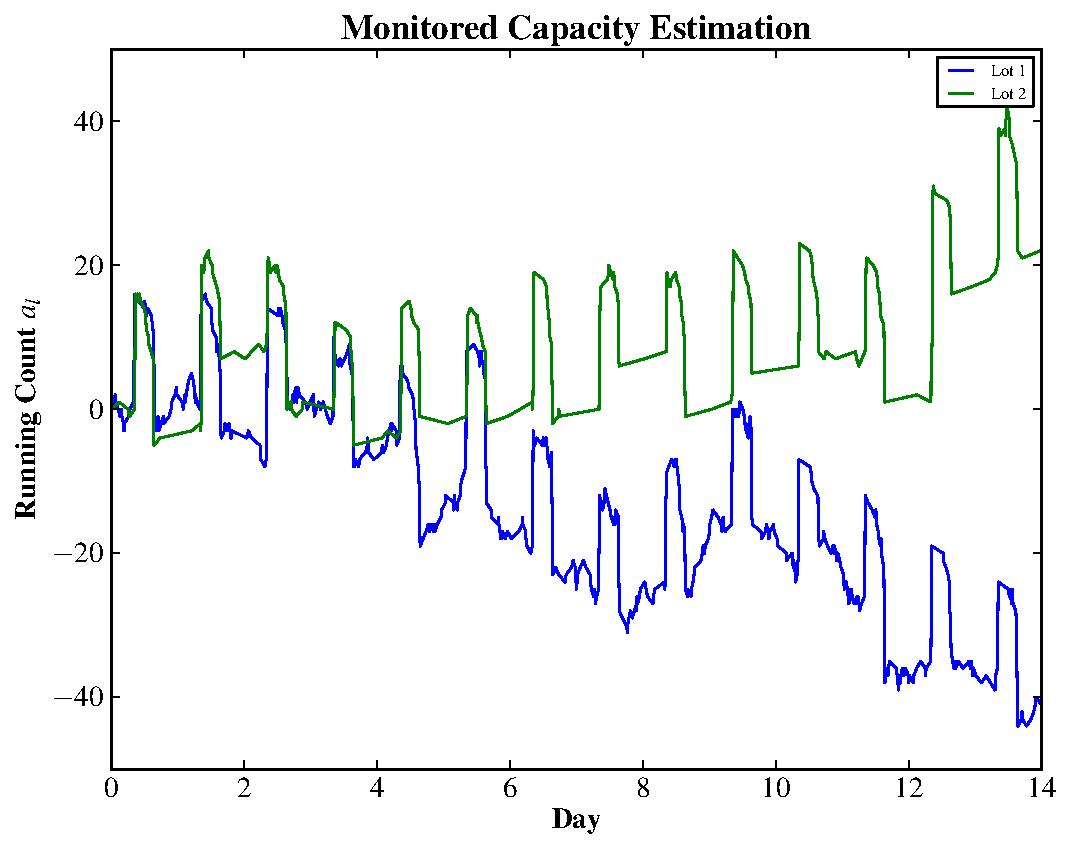
\includegraphics[width=\columnwidth]{./simulator/figures/capacity.pdf}

\caption{\textbf{Example of capacity estimation.} Running counts for two lots
are shown.}

\vspace*{-0.2in}
\label{fig-capacityexample}
\end{figure}

\subsection{Hidden Driver Estimation}

Monitored PocketParker users compete for parking spaces with unmonitored
users, which we call \textit{hidden drivers}. While we assume that
PocketParker users are generally representative of the entire driving
population, we do not assume that all or even a large fraction of drivers
will download and install PocketParker. We want our system still to provide
accurate predictions with the limited information caused by hidden drivers.
To accomplish this, PocketParker needs to estimate the percentage of drivers
that are monitored, which we call the \textit{monitored fraction} $f_m$. A
low monitored fraction indicates that few users are using PocketParker,
and vice versa. Put another way, the amount
of uncertainty PocketParker faces when predicting availability is
inversely-proportional to the monitored fraction.

\subsubsection{Importance of monitored fraction estimation}

Two examples will illustrate why we need this information and how it is used.
First, when a monitored driver leaves a parking lot, the monitored fraction
determines how long PocketParker will predict that a spot in that lot is
available. As the monitored fraction increases, the probability of
PocketParker seeing the arrival into the lot that occupies that spot
increases, and we can increase the amount of time that we estimate a spot is
available. On the other hand, as the monitored fraction decreases we see
fewer arrivals and are faced with more uncertainty. Hence, PocketParker
reduces the amount of time it predicts the spot is available. Second,
PocketParker uses the arrival and departure rates of monitored drivers to
estimate changes to parking lot availability over time. Here we must scale
the observed number of events to the actual number of events, which requires
an estimate of the monitored fraction.

PocketParker estimates the monitored fraction by first determining the
monitored capacity---the capacity of the lot measured by monitored
drivers---and then using our estimate of the lot capacity. Specifically,
given a lot with capacity $C$, the monitored fraction can be estimated as
$f_m = \frac{C_m}{C}$. Our task then becomes estimating the monitored
capacity $C_m$. To estimate the monitored capacity we maintain a running
count $a$ for each lot, decremented when drivers arrive and incremented when
they leave. We can consider $a$ as a estimate of the number of spots
available in the lot scaled by $f_m$, although we do not bound $a$ as $0 \le
a \le C$.

Figure~\ref{fig-capacityexample} shows an example of the running count for
two related lots over seven days using data generated by our lot simulator
described in more detail in the evaluation. Both lots have capacity 200 and
the actual monitored fraction is 0.1. As the data shows, the running count
experiences long-period (greater than one day) fluctuations due to events
missed by our event detector and the randomness associated with the small
percentage of drivers being monitored. However, the data also contains
short-period (less than one day) fluctuations caused by the dynamics of the
lot being monitored, and these fluctuations are roughly the size of the
monitored capacity $C_m$, which in this case is 20 spots.

This observation motivates the design of our monitored capacity estimator.
First, we bin the data into 24~hour intervals. Next, we identify the largest
availability swing over each window. Finally, we average multiple swings
together for a period of days to determine the final estimate. This simple
approach works well on lots that fill on a regular basis. For the example in
Figure~\ref{fig-capacityexample}, our estimator estimates the monitored
capacity of lots~1~and~2 as 21.01 and 21.08, respectively, within 10\% of the
true value in both cases. We perform a further analysis of our capacity
estimator using multiple lot simulations in the evaluation.

For lots that do not fill regularly, we may need to produce a
weighted sum where larger swings are weighted more heavily given our
assumption that they more accurately measure the true monitored lot capacity. 
Another approach is to use the $f_m$ estimated at
desirable lots for a given destination, which are more likely to fill
completely and often, to estimate the $f_m$ for
lesser desirable lots. Here we are making the reasonable assumption that lots
connected to the same destination share similar fractions of PocketParker
users. Finally, PocketParker's monitored fraction estimator runs periodically
to incorporate changes in the monitored fraction caused by increasing use of
PocketParker.

\subsection{Rate Estimation}

When PocketParker receives arrival and departure event information, it knows
something concrete about the state of the lot. However, to predict
availability at other times we need to adjust our estimation based on
recently-observed events, which we call rate estimation. To estimate the rate
of events in the entire population including hidden drivers, PocketParker
must scale its rate of parking events by monitored drivers appropriately.
Next, we use these scaled estimates to adjust the probability that a lot has
a certain number of spots and spots available.

During a time interval $t_0$ to $t_1$, PocketParker will observe some number
of searches $s_{obs}(t_0, t_1)$ or departures $d_{obs}(t_0, t_1)$ in any
given lot\footnote{Without loss of generality our examples of scaling and
estimating rates use notation for the search rate.}. Note that the search
count includes both arrivals---successful searches---and implicit
unsuccessful searches derived from arrivals at related lots as explained
above. However, depending on the monitored fraction $f_m$ the true count
$s_{true}(t_0, t_1)$ is likely to be much larger. Rather than simply scaling
the count by $\frac{1}{f_m}$, we want to determine the probability
distribution over all possible true counts given the rate we observed and the
estimated monitored fraction. One reason we do not simply scale by
$\frac{1}{f_m}$ is that our uncertainty about the true count should be
affected by $f_m$. If all drivers use PocketParker, we know the true count
exactly; if few do, we should be uncertain.

To compute the probability distribution we treat $s_{obs}$ as the output of a
binomial distribution with probability $f_m$ and vary the number of trials.
The binomial distribution reflects the fact that drivers are either monitored
by PocketParker or not with estimated probability $f_m$. Specifically:
%
\[
%
P(s_{true}| s_{obs}) = C \cdot {s_{obs} \choose s_{true}}
f_m^{(s_{obs})} \cdot (1 - f_m)^{(s_{true} - s_{obs})}
%
\]
%
where $C$ is a renormalization constant equal to $\sum_{s_{true}} P$.

\subsubsection{Updating the count probabilities}

Given the probability that a lot has $n$ free spots at time $t_0$, $P(t_0,
n)$, we want to estimate the probabilities $P(t_1, n)$ at a later time $t_1$.
PocketParker uses recently-observed arrivals, implicit searches and
departures to estimate the search $s_{est}$ and departure $d_{est}$ rates the
lot experienced between $t_0$ and $t_1$. Currently, we use arrival and
departures over a fixed-size window $I$ before $t_0$, $s_{obs}(t_0 -
I, t_0)$ scaled to the length of $t_0$ to $t_1$:
%
\[s_{est}(t_0, t_1) = s_{obs}(t_0 - I, t_0) \cdot \frac{(t_1 - t_0)}{I} \]
%
The value of $s_{est}(t_0, t_1)$ is then scaled as described above to
determine the distribution of $s_{true}$.  Given the predictable traffic flows
of our campus environment over the course of a term, PocketParker assumes the
rates experienced over the last $I$ time interval will continue. It may be
possible to perform better rate estimation by using historical information,
but this is left as future work.

The distribution of search rates $s_{true}(t_0, t_1)$ represents the
probabilities that the number of available spots in the lot will decline,
whereas the departure rate $d_{true}(t_0, t_1)$ represents the probability
the number of spots will increase due to departures. The convolution of $-1
\cdot s_{true}$ and $d_{true}$, $\Delta(t_0, t_1)$, represents the change in
the number of spots produced by the specific combination of arrival and
departure rates. A further convolution of $\Delta(t_0, t_1)$ with $P(t_0,
n)$ produces $P(t_1, n)$, the probability at $t_1$:
%
\[ P(t_1, n) = P(t_0, n) * (-1 \cdot s_{true}(t_0, t_1) * d_{true}(t_0,
t_1)) \]
%
where $*$ represents the discrete convolution.

Note that the convolution of $P$ with $\Delta$ can cause non-zero
probabilities in $P$ that violate our boundary conditions, namely that
$P(n < 0) = 0$ and $P(n > C) = 0$ where $C$ is the estimated capacity of
the lot. To correct this, we simply set $P(n = 0) = \sum_{n < 0} P(n)$
and $P(n = C) = \sum_{n > C} P(n)$, assigning all the probability that
the lot has less that zero free spots to the zero state and all probability
that it has more than the capacity of the lot of free spots to the empty
state.

\subsubsection{Rateless spreading}

If the departure rate exceeds the arrival rate, the probability mass of
$\Delta$ will lie primarily to the positive side and it will shift $P$ in the
positive direction, producing higher probabilities that spots are available
in the lot and lowering the probability that the lot is full. The opposite is
true when the search rate exceeds the arrival rate.

An important case is intervals during which PocketParker has observed neither
arrivals nor departures in a given lot. In this case, $\Delta$ will be
centered around $0$ but have a spread determined by the monitored fraction.
Its effect on $P$ will be to redistribute the probability mass more evenly
across the entire interval from $0$ to $C$. Taken over many intervals, the
probability of the lot having any number of spots available will equalize,
which is what we would expect: after a long period without any information,
all states become equally likely and we cannot make an accurate prediction of
the state of the lot. Note also that the speed at which the probabilities are
redistributed through rateless spreading is determined again by the monitored
fraction. The fewer drivers we monitor, the more quickly we lose all memory
of the state of the lot.

\subsection{Online Updates}

Finally, we conclude by describing how PocketParker uses arrival to adjust
its availability model instantaneously at runtime. Each arrival and departure
received at time $t$ represent strong positive information---moments when
PocketParker knows either that a spot just existed (arrival) or now exists
(departure). PocketParker uses these events to adjust the probability
distribution and incorporate this new information. 

Arrivals provide two somewhat conflicting pieces of information. First,
PocketParker knows that at the time of the arrival there was a spot free, so
in this way arrivals indicate that the lot is not full. However, PocketParker
also knows that immediately after an arrival the lot has one fewer available
spots. So we incorporate arrivals in two steps. First, we set $P(t, 0) = 0$
indicating the availability of a spot and renormalize the distribution.
Second, we shift the entire distribution downward by one spot, $P(t, n) =
P(t, n - 1)$, reflecting the loss of a parking space due to the arrival.

Departures produce a straightforward change to the probability distribution.
When a user departs, we know at that moment that there is a free spot in the
lot, so we can set $P(t, 0) = 0$ and renormalize the distribution. Note that,
since the probability that the lot is free is $P_{free} = \sum_{n > 0} P(t,
n)$, at the exact time of each departure the probability that a spot is free
is equal to 1. 

Unsuccessful implicit searches, in contrast, represent weaker negative
information, both because they were not observed by PocketParker and so may
not have actually taken place, or because they may not have been thorough.
What we want is to increase the probability that the lot is full while
reflecting our current estimate of the lot. We do this by shifting the
availability distribution towards full by some amount $s$, which we refer to
as the \textit{search shift parameter}. So, after an implicit unsuccessful
search, we set $P(t, n) = P(t, n - s)$, with $P(t, 0) = \sum_0^s P(t, n)$.
The search shift parameter determines how aggressively PocketParker will use
information provided by implicit searches.

\subsubsection{Weighted arrivals and departures}

Shifting the distribution one space on arrivals and departures is the most
conservative approach representing what we definitely know: that one spot is
available. However, if we assume that our monitored drivers are
representative of some larger number of hidden drivers, we may set $P_l(t, n
< X) = 0$ for some $X$ larger than 1 and scaling with $\frac{1}{f_m}$. For
our experiments we choose the conservative approach and set $X = 1$. As
future work we consider how users may customize the behavior of PocketParker
to be more or less aggressive in locating parking spots, trading off time for
a better spot.

% flatex input end: [model.tex]

% flatex input: [evaluation.tex]
\begin{figure*}[t]
\centering
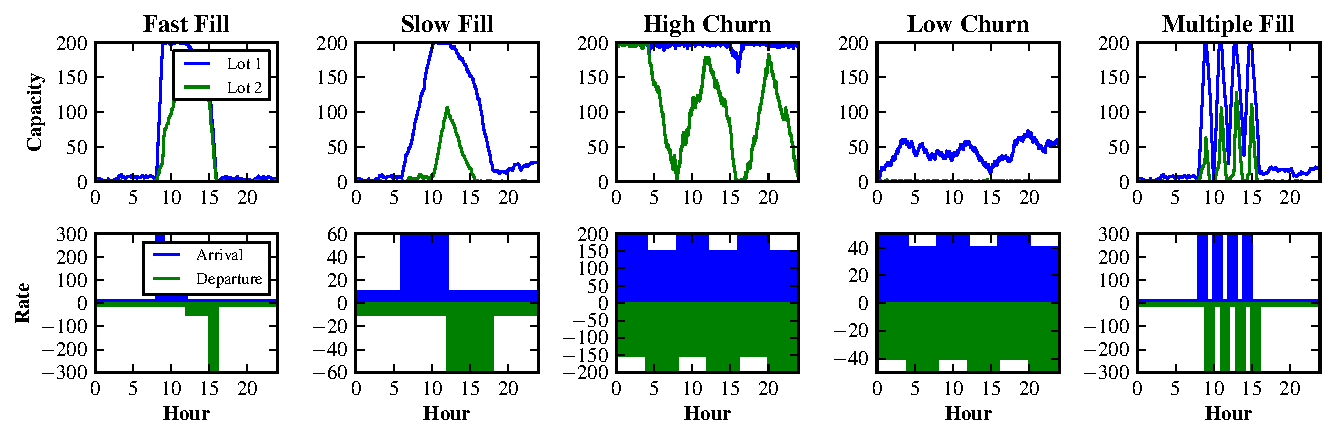
\includegraphics[width=\textwidth]{./simulator/figures/lots.pdf}

\caption{\textbf{Description of each type of lot simulated.} Five different
lots with different behaviors were used.}

\label{fig-lotsdescription}
\end{figure*}

\newpage

\section{Evaluation}

We evaluated PocketParker in three ways. First, we conducted a controlled
experiment to determine the best parameter settings for our event detector.
Second, we implemented a parking lot simulator to experiment with various
kinds of lots under differing monitored fractions. Finally, we deployed
PocketParker on our campus. We monitored two lots with camera monitoring to
ground truth our predictions. Our evaluations confirm that PocketParker is
efficient and accurate.

\subsection{Detector Experiment}

% flatex input: [./figures/experiment_table/table.tex]
\newcolumntype{b}{>{\hsize=1.4\hsize}X}
\newcolumntype{s}{>{\hsize=.6\hsize}X}
\begin{table}[t]
{\small
\begin{threeparttable}
\begin{tabularx}{\columnwidth}{b s b s}
  {{\textbf{Carry Location}}} & {{\textbf{Count}}} &
  {{\textbf{Car Location}}} &
  {{\textbf{Count}}} \\
 \hline
In hand & 18 & Cup holder & 16 \\
Side bag & 10 & Car seat  & 9 \\
Back pack & 10 & Side bag & 10 \\
In hand talking & 7 & Back pack & 9 \\
Front pocket & 14 & Front pocket & 14 \\
Jacket pocket & 14 & Jacket pocket & 14 \\
Back pocket & 7 & Back pocket & 14 \\
\end{tabularx}
\end{threeparttable}
\caption{\textbf{Carry and car location for detector experiment.}
Eight participants generated 80 runs, carrying and placing the
phone in their car in many ways.}
\label{table-experiment}
}
\vspace*{-0.1in}
\end{table}

% flatex input end: [./figures/experiment_table/table.tex]


To determine the right parameter settings for our transition detector, we
conducted a controlled experiment. During this experiment, accelerometer and
GPS data was collected and stored continuously on each device, and
participants were asked to manually label each transition into and out of the
car. Afterwards, data was processed by a Python simulator implementing the
identical algorithm used by the PocketParker, allowing us measure
accuracy and energy consumption as a function of the detector duty cycle.

Eight volunteers participated, including seven men and one woman. Seven were
right-handed and one was left-handed. Each was asked to conduct the same
experiment ten times: (1) carrying the instrumented phone, walk to their car;
(2) label departure; (3) drive around campus briefly; (4) park and label
arrival; (5) return inside. Since the way the phone is carried while walking
and placed in the car while driving affects the accelerometer readings, care
was taken to generate a good mix of carry and car location styles.
Table~\ref{table-experiment} shows the breakdown. The experiment permitted us
to obtain sensing data from a cross section of individuals possessing
different body morphologies, habits of driving cars, and ways of handling
mobile devices.

Figure~\ref{fig-energy} displays the tradeoff between energy usage and
detection accuracy as a function of the PocketParker duty cycle. Here we
combine an active period of 5s with a inactive period of variable length,
between 5~and~55s, for an overall duty cycle between 0.5 and 0.06. Our
simulator uses energy numbers from the Android Fuel Gauge application
to estimate average power consumption.  This graph measures the accuracy of
detected events in terms of distance from the actual location of the event
labeled by the participant.

As expected, longer duty cycles consume less energy but produce longer
detection latencies which translate into higher distances from the event
location. Note also that departures have higher location error than arrivals
because departing users are driving and therefore traveling more rapidly.
Overall power usage by PocketParker is low, under 10~mW at all duty cycles.
Because PocketParker's ability to map parking events into lots is affected by
the detection distance accuracy, we chose a low total period of 15~s for a
0.25 duty cycle. This allows PocketParker to determine location to within
25~m for arrivals and 80~m for departures. Power consumption at this duty
cycle is 8~mW, representing 4.2\% of the capacity of a 1500~mAh battery over
24~hours.


\begin{figure}[t]
\centering
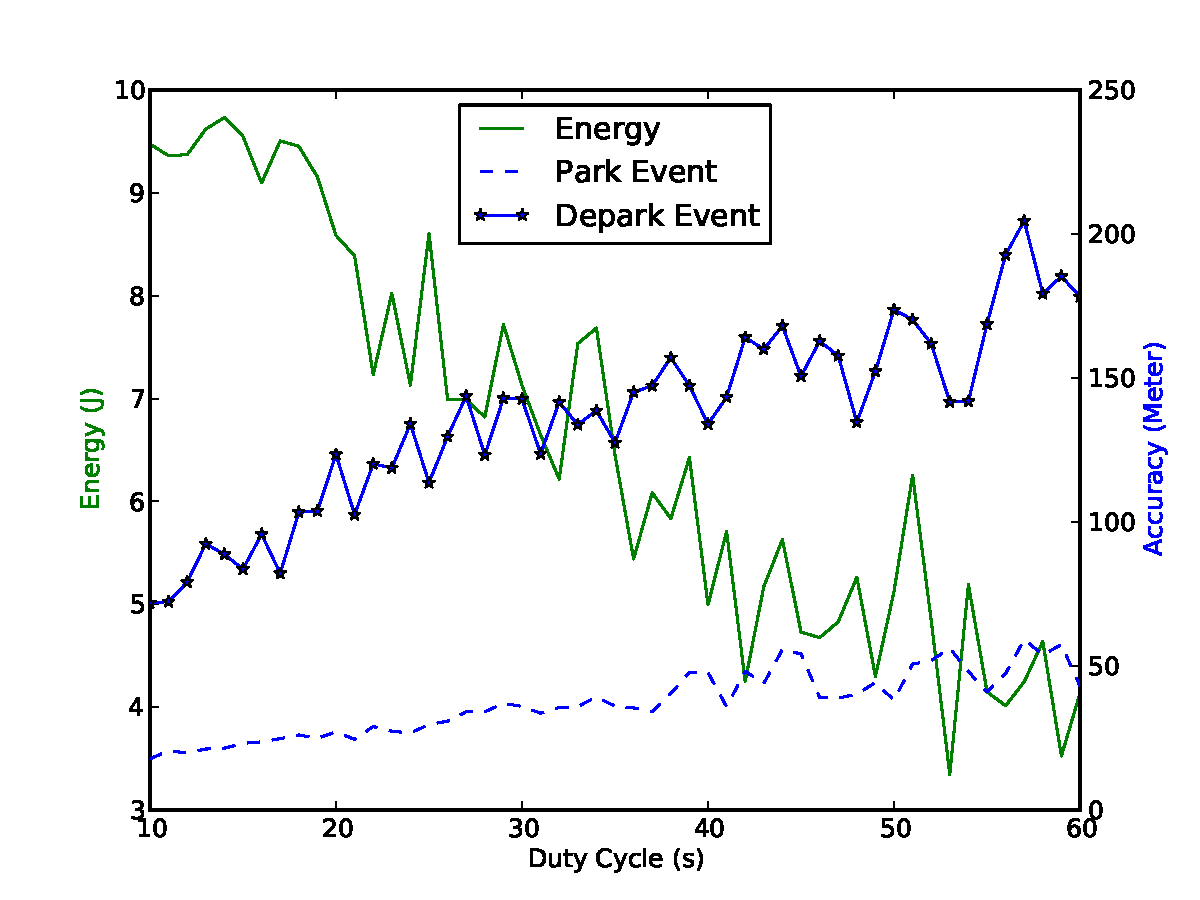
\includegraphics[width=\columnwidth]{./figures/Energy_accuracy.pdf}

\caption{\textbf{Power usage vs. detector accuracy.} Energy usage by
PocketParker is low at all duty cycles, so we chose a high duty cycle to
improve accuracy.}

\label{fig-energy}
\end{figure}

Using the same data we also examine the false positive and negative rates for
arrivals and departures. This is important since, without explicit user
input, it would be impossible to determine this information while
PocketParker is in use. Figure~\ref{fig-falsepositives} shows PocketParker
can detect 80\% of arrival and departure events correctly at the 0.25 duty
cycle we use. False positive rates are already quite low, and this is before
we apply our GPS availability filter and lot location filters. False
positives decline as the duty cycle decreases because PocketParker has fewer
opportunities to detect user activity.
\begin{figure}[t]
\centering
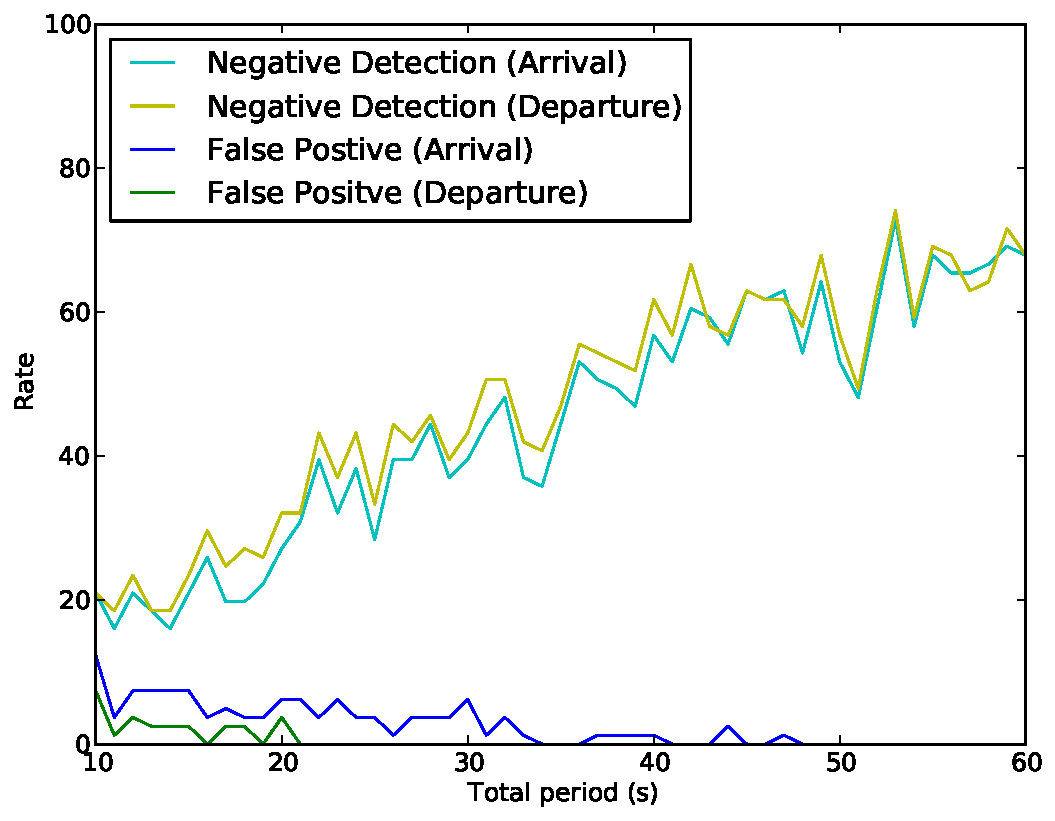
\includegraphics[width=\columnwidth]{./figures/Rate_FP_and_ND.pdf}

\caption{\textbf{False positive and negative rates as a function of detector
duty cycle.}} 

\label{fig-falsepositives}
\end{figure}

\subsection{Simulation Results}

To experiment with PocketParker in a more controlled setting, we implemented
a parking lot simulator in Python. Our simulator allows us to simulate any
number of parking lots associated with any number of points of interest with
varying desirability levels. For simplicity during our evaluation, we
simulate two lots 1~and~2 with lot~1 filling before lot~2, although lot
choice by simulated drivers is randomly weighted. Particularly for evaluating
our monitored fraction estimation, we use five types of lots that fill and
empty differently:

\begin{itemize}

\item \textbf{Fast Fill} and \textbf{Slow Fill} fill once per day quickly or
slowly, like a lot associated with a place of work.

\item \textbf{Multiple Fill} represents a lot that rapidly fills and empties
repeatedly during each day, like a campus lot or movie theater.

\item \textbf{High Churn} starts with lot~1 full and experiences continuously
high arrival and departures rates, like an airport parking lot.

\item \textbf{Low Churn} represents underutilized lots that never completely
fill, with lot~2 almost completely unused.

\end{itemize}

Figure~\ref{fig-lotsdescription} shows the arrival and departure rates for
each of the types of lot as well as the resulting per-lot capacity.

\begin{figure*}
\centering
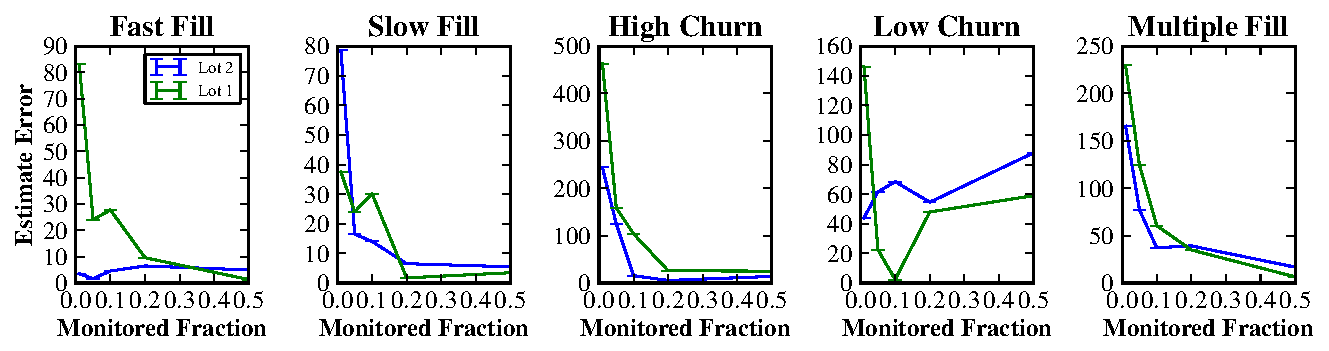
\includegraphics[width=\textwidth]{./simulator/figures/capacity_experiment.pdf}

\caption{\textbf{Errors in monitored fraction estimation.} Currently
PocketParker is better at estimating the monitored fraction when lots fill
and empty regularly.}

\label{fig-capacityerrors}
\end{figure*}

\subsubsection{Monitored fraction estimation}

Earlier we described our approach to estimated the monitored fraction, a
parameter important to the operation of the PocketParker availability
estimator. Figure~\ref{fig-capacityerrors} shows the results of 10 random
simulations for each lot type. In each case, the monitored fraction estimator
uses a weeks worth of data and proceeds as described previously. The error in
the monitored fraction estimate is shown as a function of the actual
monitored fraction for the simulation used.

For the five types of lots, we would expect PocketParker to do better
monitored fraction estimation when lots fill regularly---Fast Fill, Slow
Fill, and Multiple Fill---and poorly when they do fill erratically or not at
all---High and Low Churn. The results in Figure~\ref{fig-capacityerrors}
generally follow this pattern. Errors for High Churn are quite high, and Low
Churn errors persist even at high monitored driver fractions. This is
natural, as the Low Churn lot never fills.  By contrast, the accuracy rate for
the Fast, Slow and Multiple Fill models improve with an increasing fraction of
monitored drivers.

\subsubsection{Probability and availability}

We now consider how PocketParker adjusts lot availability probabilities.  It
uses these probabilities to rank available lots in response to queries.
Figure~\ref{fig-trackingexample} shows a 24~hour simulation of a Fast Fill
parking lot with a monitored fraction of 0.1 and a 10\% error in the
estimation of the monitored fraction. The ground truth capacity of the lot as
simulated is plotted next to the PocketParker probability that the lot has an
available spot. At the beginning, both lots are marked as free. After lot~1
fills and lot~2 begins to fill, which generates implicit searches
in lot~1, the availability probability of lot~1 drops. It spikes upward
repeatedly due to departures from lot~1---which reset the short-term
probability of an available spot back to 1---but does not equal the
probability for lot~2 again until the point when the departure rate for lot~1
climbs.

\subsubsection{Prediction accuracy}

\begin{figure}[t]
\centering
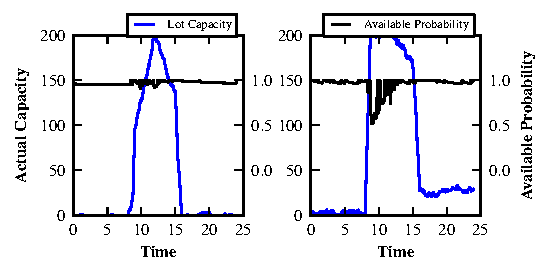
\includegraphics[width=3.325in]{./simulator/figures/tracking_fastfill_horizontal.pdf}

\caption{\textbf{Availability probabilities tracking lot capacity.} Dips in
the availability probability correspond to times when PocketParker believes
the lot is full. Discontinuities are caused by departures, which set the
instantaneous probability that the lot is available to 1.0.}

\label{fig-trackingexample}
\end{figure}
PocketParker exists to help drivers park efficiently.  To examine its
prediction accuracy, we have PocketParker rank two model lots in order of
preference at regular timesteps and then compare these results with the ground
truth from a simulator.  Finally, we categorize the results as a correct
prediction, a missed opportunity---a case where a more desirable lot was
available than the one that PocketParker recommended---or a waste of
time---where PocketParker sent the user to a full lot.
Table~\ref{table-accuracy} shows data results from simulations run using
varying monitored fractions$f_m$ of drivers.

Also, Figure~\ref{fig-accuracy} shows that several trends can be observed in
the results. First, overall PocketParker does well on most lot types. The
High Churn lot presents the greatest difficulty, which we would expect since
its large number of incoming and outgoing drivers make prediction difficult.
We are also concerned that the High Churn errors are largely waste of time
errors, indicating that PocketParker is frequently sending drivers to the
wrong lot. This is likely because it is predicting that spots are available
longer than they actually are. Clearly more work is needed to determine the
right approach for High Churn lots, and this type of lot may be a better fit
for infrastructure-based solutions.
% flatex input: [./simulator/figures/accuracy_table.tex]
\begin{table}[t]
\begin{threeparttable}
{\small
\begin{tabularx}{\columnwidth}{Xccrrrr}
\multicolumn{1}{c}{\textbf{Type}} & 
\multicolumn{1}{c}{\textbf{Day}} & 
\multicolumn{1}{c}{\textbf{$f_m$}} & 
\multicolumn{1}{c}{\textbf{Correct}} & 
\multicolumn{1}{c}{\textbf{Missed}} & 
\multicolumn{1}{c}{\textbf{Waste}}\\ \toprule

\textbf{Campus} & 1 & 0.07 & 56.1 \% & 43.9 \% & 0.0 \% \\
& 2 & 0.13 & 80.9 \% & 1.9 \% & 17.2 \% \\
& 3 & 0.17 & 72.4 \% & 11.0 \% & 16.6 \% \\
& 4 & 0.20 & 94.2 \% & 5.8 \% & 0.0 \% \\
\end{tabularx}
}
\caption{\textbf{Accuracy of PocketParker predictions for various fraction of monitored drivers for 4 days.}}
\label{table-accuracy}
\end{threeparttable}
\end{table}

% flatex input end: [./simulator/figures/accuracy_table.tex]

% error in the

Excluding the High Churn lot, the lot with the lowest correct percentage with
a $f_m > 0.1$ is 80\% for the Slow Fill lot.  Accuracy above
this $f_m$ is consistently good for all lots save the High Churn model.  The
Low Churn lot does have a small number of errors but this is because both
lots are usually empty. An unavoidable lower bound to accuracy is imposed by
the frequency of parking PocketParker has the most information about lot
availability during periods of parking events. Once such information stops,
prediction uncertainty grows. Thus, to the degree that PocketParker queries
follow a pattern of arrivals and departures, it will do well.

\begin{figure}[t]
\centering
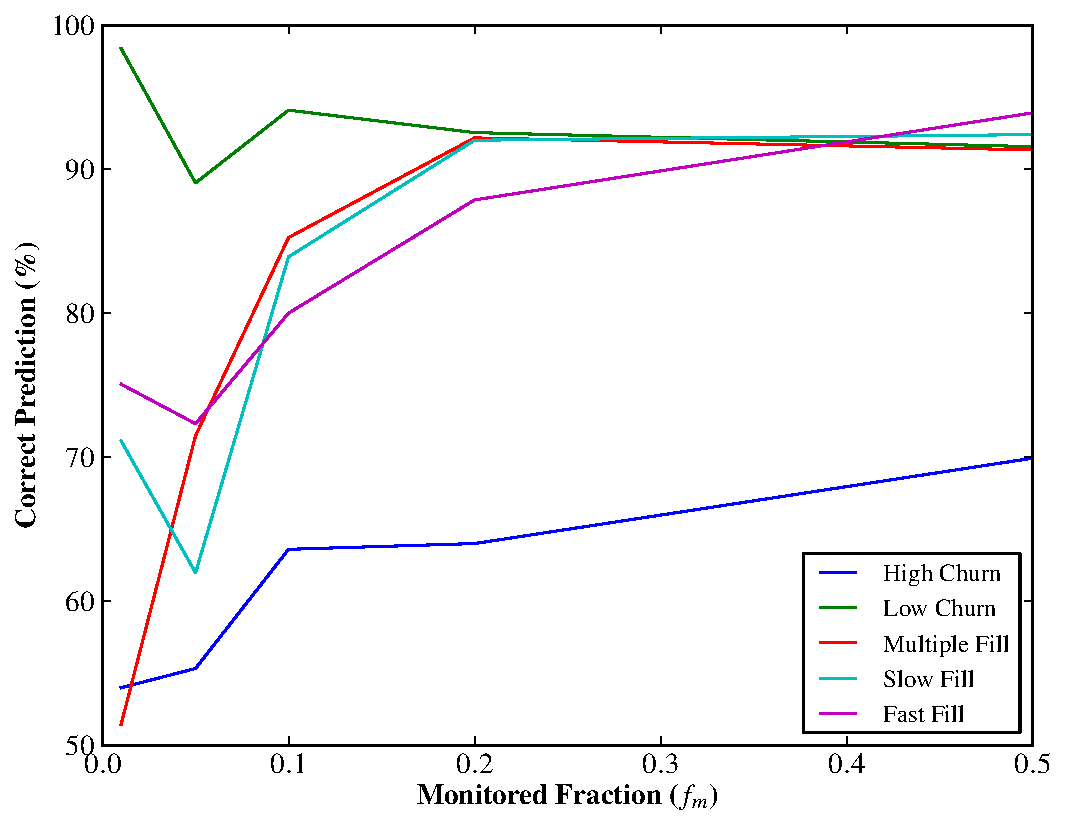
\includegraphics[width=\columnwidth]{./simulator/figures/accuracy_graph.pdf}

\caption{\textbf{Accuracy predictions for various kind of lots and parameters.}}
\label{fig-accuracy}
\end{figure}

\newpage
\vspace*{-0.4in}
\subsection{Deployment}

\begin{figure}[t]
\centering
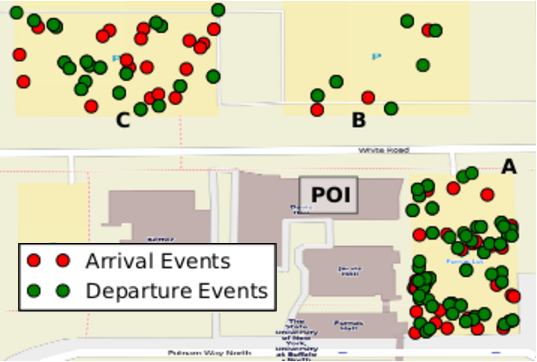
\includegraphics[width=\columnwidth]{./figures/smallEventsOnThreeParkingLot.pdf}

\caption{\textbf{Map showing 217~parking events detected by PocketParker
during our forty-five-day deployment in three key lots.} Lot~A is considered
the most desirable, and Lots~A~and~B were monitored by cameras to establish
ground truth.}

\label{fig-events}
\end{figure}

Finally, to establish the accuracy of PocketParker we deployed our PocketParker
application on \PhoneLab{}~\cite{phonelab-testbed} after obtaining IRB approval. The only
infrastructure required was the PocketParker server for receiving events and
generating availability estimates. The userbase involved 105 total participants
from \PhoneLab{}.  Over 45 days of monitoring, the PocketParker app  run by
these users
generated \num{10827} events---5916 arrivals and 4911 departures---for an
average of 241 per day. Our main and medical campuses produced 3645 and 846
total events respectively, with non-campus locales contributing to the
remaining 6336 events.

Figure~\ref{fig-events} shows all of the events that occurred in three key
lots that we monitored during our experiment. Our computer science building
is labeled as the point of interest (POI). The three labeled lots were
assigned our building as a destination and desirability indices based on
their proximity. To determine ground truth availability, we positioned four
cameras at locations within the building to monitor lots A~and~B in
Figure~\ref{fig-events}. Despite the fact that many parking events took place
in lot~C, we were unable to locate a suitable vantage point to gather camera
data for that lot. Nexus~S~4G smartphones equipped with fish-eye lenses took
\num{34138} time lapse images each minute for four days. 
%and uploaded them to a central server.

Using these images, we produced lot capacity charts containing the proportion
of free spots in a given lot at a given time. Specifically, we
hand coded the images for the two lots at ten minute intervals. We were
particularly interested in the transition between empty and full states, so we
were careful to ensure that a lot was never marked full even if
there was a single available spot.

We fed these capacity charts, along with parking events in camera-monitored
lots A~and~B, into the PocketParker estimation engine to produce accuracy
results for a four day period.  Table~\ref{table-accuracy} shows results for
our campus deployment. Overall the accuracy of PocketParker is excellent,
achieving 94.2\% accuracy at a monitored driver fraction of 0.2, which we
believe is an accurate estimate of the percentage of PocketParker users using
these lots.

% flatex input end: [evaluation.tex]

% flatex input: [future.tex]
\section{Limitations and Future Work}

The pocketsourcing approach taken by PocketParker makes it easy to integrate
into existing mapping applications, which would provide access to the estimated
half-billion smartphone users that have installed Google Maps. The increase in
the monitored fraction would significantly improve
PocketParker's accuracy and usability. This would enable PocketParker to display
the location of the events more precisely.
%PocketParker can make use of the frequent
%GPS updates needed by the mapping application to provide information about exact
%location of the event.

PocketParker presently bases its parking predictions on a fifteen-minute
limited rolling window of recent parking events. We do not presently tap the
benefit of daily and weekly patterns that would otherwise enhance predictive
accuracy, but hope to do so in the future. Maintaining a historical data
collected from our own application would increase
the sample size and hence statistical accuracy of our parking predictions.
This is another area where integration with a mapping application would help,
providing PocketParker with access to much more data.

Presently, PocketParker is designed for a single user per vehicle. Proximity
detection of users would allow the system to detect the case of
multiple users in a vehicle and thus to reduce spurious arrival and departure
events.

Finally, we believe that once users begin interacting with PocketParker we
will see different parking preferences emerge. Some user will want
PocketParker to help them aggressively hunt for spots, and be willing to wait
for drivers to leave. Others may be more interested in simply finding a spot
quickly even if it is farther away. PocketParker has several parameters that
can control its predictions, and we will need to determine how to expose
these options to users.

%
%An anticipated future enhancement of our application, adding capacity to
%solicit the exact preferred parking destination from a user, will also
%significantly benefit from historical data. We will be able to suggest lots
%available to end users based on proximity to logistically preferable but full
%lots. If a user further furnishes insight into how long he is willing to wait
%for a desired parking location, we will be able to mine historical data for
%how long someone in that situation will have to wait for a parking spot and
%make recommendations accordingly.
%
%Integration with Google Maps or other navigation solution will permit
%automatic retrieval of labeled search preferences in lieu of manual user
%input.
%
%
%Over time, accuracy and popularity of PocketParker should mutually enhance
%each other.  Increasingly dense data, stemming from higher user adoption rates
%and additional historical information, 
%
%...will enhance accuracy, and hence credibility of the application, with end users...
%
%
%labelled searches...

% flatex input end: [future.tex]

% flatex input: [conclusions.tex]
\vspace*{-0.05in}
\section{Conclusion}

We have presented PocketParker, a pocketsourcing solution for predicting
parking lot availability. PocketParker requires no explicit user input and
can provide parking lot predictions without being removed from a user's
pocket. PocketParker's accuracy derives from combining a simple and
energy-efficient parking event detector with a sophisticated parking lot
availability model that incorporates the effect of hidden drivers that
compete with PocketParker users for parking spots. Our evaluation has
demonstrated that PocketParker can provide accurate predictions across a
variety of parking lot types and patterns, and that a fielded deployment of
PocketParker performed extremely well. We look forward to integrating
PocketParker into existing mapping applications and bringing it to pockets
everywhere.

\vspace*{-0.05in}
\section*{Acknowledgements}

The authors would like to thank the anonymous UbiComp reviewers for their
constructive feedback.

% flatex input end: [conclusions.tex]

\clearpage

\balance
{\footnotesize
%*flatex input: [paper.bbl]
\begin{thebibliography}{10}

\bibitem{car-detect}
Vehicle detection with wireless sensors, 2008.

\bibitem{parkingdesign}
{Parking Lot Design Standards}.
\newblock \url{http://goo.gl/v0F7u}, 2012.

\bibitem{sfpark}
{SFPark}.
\newblock \url{http://goo.gl/ZlxQu}, 2012.

\bibitem{openstreetmap}
{OpenStreetMap}.
\newblock \url{http://www.openstreetmap.org/}, 2013.

\bibitem{Chen:2012:COS}
Chen, X., Santos-Neto, E., and Ripeanu, M.
\newblock Crowdsourcing for on-street smart parking.
\newblock In {\em Proceedings of the second ACM international symposium on
  Design and analysis of intelligent vehicular networks and applications},
  DIVANet '12, ACM (New York, NY, USA, 2012), 1--8.

\bibitem{Constandache:2010:DYS}
Constandache, I., Bao, X., Azizyan, M., and Choudhury, R.~R.
\newblock Did you see bob?: human localization using mobile phones.
\newblock In {\em Proceedings of the sixteenth annual international conference
  on Mobile computing and networking}, MobiCom '10, ACM (New York, NY, USA,
  2010), 149--160.

\bibitem{mstp-park}
Corporation, H.
\newblock Advanced parking information system evaluation report, 2001.

\bibitem{Delot:2009:CRP}
Delot, T., Cenerario, N., Ilarri, S., and Lecomte, S.
\newblock A cooperative reservation protocol for parking spaces in vehicular ad
  hoc networks.
\newblock In {\em Proceedings of the 6th International Conference on Mobile
  Technology, Application and Systems}, Mobility '09, ACM (New York, NY, USA,
  2009), 30:1--30:8.

\bibitem{Keally:2011:PTP}
Keally, M., Zhou, G., Xing, G., Wu, J., and Pyles, A.
\newblock Pbn: towards practical activity recognition using smartphone-based
  body sensor networks.
\newblock In {\em Proceedings of the 9th ACM Conference on Embedded Networked
  Sensor Systems}, SenSys '11, ACM (New York, NY, USA, 2011), 246--259.

\bibitem{5062057}
Lu, R., Lin, X., Zhu, H., and Shen, X.
\newblock Spark: A new vanet-based smart parking scheme for large parking lots.
\newblock In {\em INFOCOM 2009, IEEE} (2009), 1413--1421.

\bibitem{Mathur:2010:PDS}
Mathur, S., Jin, T., Kasturirangan, N., Chandrasekaran, J., Xue, W., Gruteser,
  M., and Trappe, W.
\newblock Parknet: drive-by sensing of road-side parking statistics.
\newblock In {\em Proceedings of the 8th international conference on Mobile
  systems, applications, and services}, MobiSys '10, ACM (New York, NY, USA,
  2010), 123--136.

\bibitem{phonelab-testbed}
Nandugudi, A., Maiti, A., Ki, T., Bulut, F., Demirbas, M., Kosar, T., Qiao, C.,
  Ko, S.~Y., and Challen, G.
\newblock Phonelab: A large programmable smartphone testbed.
\newblock In {\em Proceedings of First International Workshop on Sensing and
  Big Data Mining}, SENSEMINE'13, ACM (New York, NY, USA, 2013), 4:1--4:6.

\bibitem{Nawaz:2013:PSB}
Nawaz, S., Efstratiou, C., and Mascolo, C.
\newblock Parksense: A smartphone based sensing system for on-street parking.
\newblock In {\em Proceedings of the 19th Annual International Conference on
  Mobile Computing \& Networking}, MobiCom '13, ACM (New York, NY, USA, 2013),
  75--86.

\bibitem{propst2012embedded}
Propst, J., Poole, K., and Hallstrom, J.
\newblock An embedded sensing approach to monitoring parking lot occupancy.
\newblock In {\em Proceedings of the 50th Annual Southeast Regional
  Conference}, ACMSE'12, ACM (New York, NY, USA, 2012), 309--314.

\bibitem{Reddy:2010:UMP}
Reddy, S., Mun, M., Burke, J., Estrin, D., Hansen, M., and Srivastava, M.
\newblock Using mobile phones to determine transportation modes.
\newblock {\em ACM Trans. Sen. Netw. 6}, 2 (Mar. 2010), 13:1--13:27.

\bibitem{Wang:2009:FEE}
Wang, Y., Lin, J., Annavaram, M., Jacobson, Q.~A., Hong, J., Krishnamachari,
  B., and Sadeh, N.
\newblock A framework of energy efficient mobile sensing for automatic user
  state recognition.
\newblock In {\em Proceedings of the 7th international conference on Mobile
  systems, applications, and services}, MobiSys '09, ACM (New York, NY, USA,
  2009), 179--192.

\bibitem{Yang:2011:DDP}
Yang, J., Sidhom, S., Chandrasekaran, G., Vu, T., Liu, H., Cecan, N., Chen, Y.,
  Gruteser, M., and Martin, R.~P.
\newblock Detecting driver phone use leveraging car speakers.
\newblock In {\em Proceedings of the 17th annual international conference on
  Mobile computing and networking}, MobiCom '11, ACM (New York, NY, USA, 2011),
  97--108.

\end{thebibliography}

% flatex input end: [paper.bbl]
%FLATEX-REM:\bibliographystyle{acm-sigchi}
%FLATEX-REM:\bibliography{references}
}

\end{document}

% flatex input end: [paper.tex]
